\pagebreak\section{Blinking \& Fading LED}

\subsection{Blinking LED}
LEDs are small, powerful lights that are used in many different applications. To start, we will work on blinking an LED, the Hello World of microcontrollers. It is as simple as turning a light on and off. Establishing this important baseline will give you a solid foundation as we work towards experiments that are more complex.

\subsubsection{Experiment URL}
     Use this \href{https://www.tinkercad.com/things/cJh2vPJHNMo?sharecode=pHXIFXpJnKTcQPuxdNKi-4YMURyigVNB9XbDgZYDrw8}{link} to get the \textbf{Tinkercad} simulation of this experiment.
    
\subsubsection{Objectives}
In this lesson, we will program the Arduino's GPIO output high level and low level (0V), and then make
the LED which is connected to the Arduino’s GPIO flicker with a certain frequency

\subsubsection{Necessary Components}
We will need the following components −
\begin{itemize}
    \item 1 x Breadboard
    \item 1 x Arduino Uno R3
    \item 1 x LED
    \item 1 x 330 $\Omega$ Resistor
    \item 2 × Jumper
\end{itemize}

\pagebreak\subsubsection{Circuit Diagram}
        \begin{figure}[!ht]
            \centering
            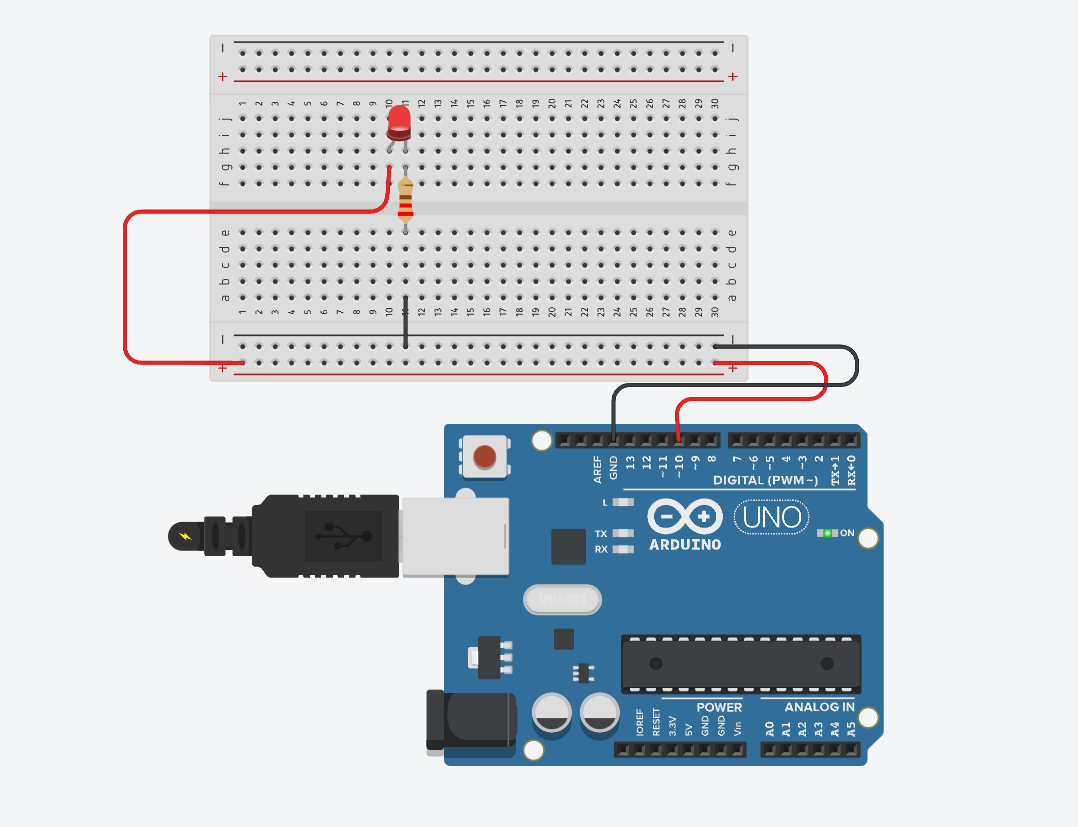
\includegraphics[width =0.75\textwidth]{images/BlinkingLED.png}
        %    \caption{Blinking LED circuit}
        \end{figure}
            
\subsubsection{Arduino Code}
    \begin{lstlisting}[style = Arduino]
    /* Blinking LED   */

int  ledPin = 10; //Initialize digital pin 10 set as LED output pin
int gap = 500; // Wait for 500 millisecond(s)

void setup()
{
  pinMode(ledPin, OUTPUT);
}

void loop()
{
  // turn the LED on (HIGH is the voltage level)
  digitalWrite(ledPin, HIGH);
  delay(gap); 
  // turn the LED off by making the voltage LOW
  digitalWrite(ledPin, LOW);
  delay(gap);
}
    \end{lstlisting}
 
\begin{comment}
\subsubsection{Conclusion}    
    We should see our LED turn on and off with the given delay. If the required output is not seen, we need to make sure we have assembled the circuit correctly, and have verified and uploaded the code to the board.
\end{comment}    
    
%%%%%%%%%%%%%%%%%%%%%%%%%%%%%%%%%%%%%%%%%%%%%%%%%%%%%%%%%%%%%%%%%%%%%%%%%%%%%%%%%%%%%%%%%%%%%%%%%%%%%%%%%%%%%%%%%%%%%%%%%%%
%%%%%%%%%%%%%%%%%%%%%%%%%%%%%%%%%%%%%%%%%%%%%%%%%%%%%%%%%%%%%%%%%%%%%%%%%%%%%%%%%%%%%%%%%%%%%%%%%%%%%%%%%%%%%%%%%%%%%%%%%%%

\pagebreak\subsection{Fading LED}

\subsubsection{Experiment URL}
Use this \href{https://www.tinkercad.com/things/dPLO4csum3h?sharecode=fTlXe0aOvAKUaa1xymJ71oC1m0_NHLRisRVjCh7YtyI}{link} to get the \textbf{Tinkercad} simulation of this experiment.
        
\subsubsection{Objectives}
This experiment demonstrates the use of the analogWrite() function in fading an LED off and on. AnalogWrite uses pulse width modulation (PWM), turning a digital pin on and off very quickly with different ratio between on and off, to create a fading effect.
\subsubsection{Necessary Components}
We will need the following components −
\begin{itemize}
    \item 1 x Breadboard
    \item 1 x Arduino Uno R3
    \item 1 x LED
    \item 1 x 330 $\Omega$ Resistor
    \item 2 × Jumper
\end{itemize}
\subsubsection{Schematic}
        \begin{figure}[!ht]
            \centering
            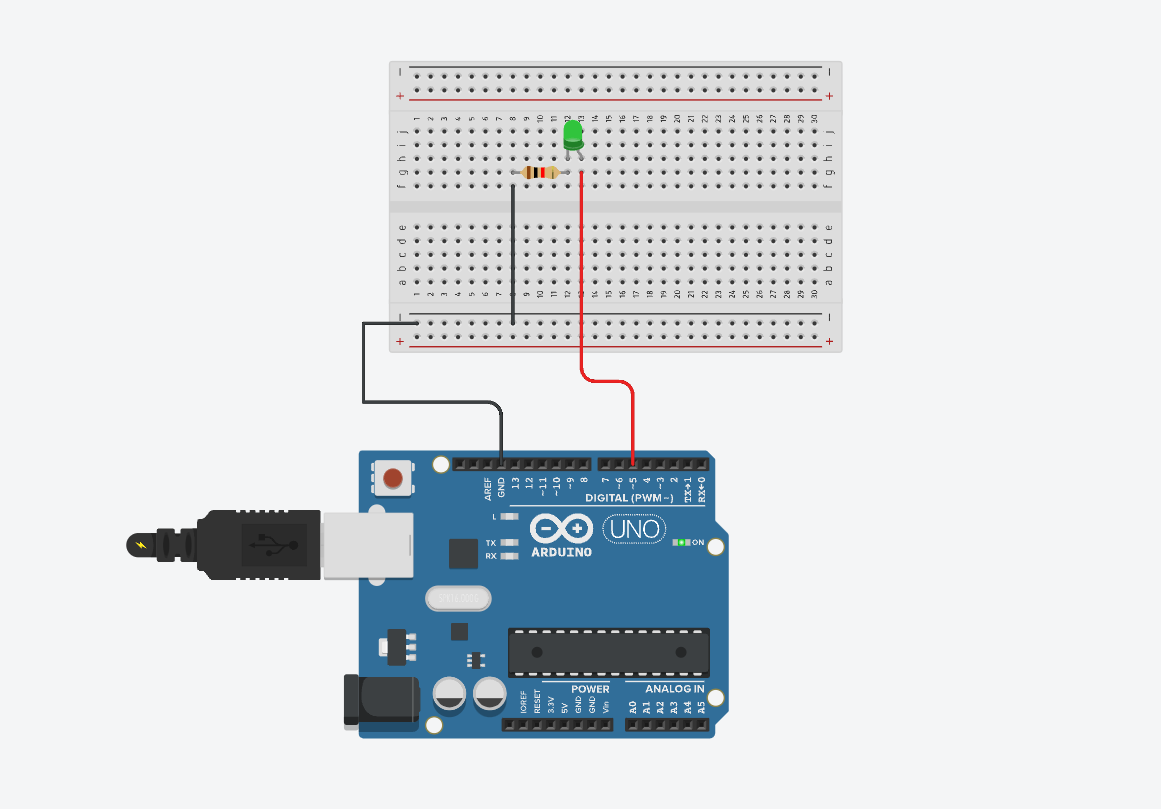
\includegraphics[width =0.75\textwidth]{images/FadingLED.png}
    %        \caption{Fading LED circuit}
        \end{figure}
            
\pagebreak\subsubsection{Arduino Code}
    \begin{lstlisting}[style = Arduino]
/*Fading LED*/

const int pinLED = 5; //declaring PWM pin 5 as LED output
int brightness = 0 ; //declaring LED initial condition
int fadeAmount = 5; // how many points to fade the LED by

void setup()
{
  pinMode(pinLED, OUTPUT); //initializing PWM pin 5 as LED output
  Serial.begin(9600);
}

void loop(){

  for (brightness = 0; brightness <= 255; brightness += fadeAmount){
  analogWrite(pinLED,brightness);
  delay(50); //interval for the brightenig effect
	}
	
  delay(500);  //wait for 500ms to run the loop again
  
  for (brightness = 255; brightness >= 0; brightness -= fadeAmount){
  analogWrite(pinLED,brightness);
  delay(50); //interval for the dimming effect
	}
  delay(500); //wait for 500ms to run the loop again
}\end{lstlisting}